\documentclass[11pt]{article}
\usepackage[margin=1in]{geometry}
\usepackage[utf8]{inputenc}
\usepackage[T1]{fontenc}
\usepackage{amsmath,amssymb}
\usepackage{mathtools}
\usepackage{graphicx}
\graphicspath{{figures/}}
\usepackage{booktabs}
\usepackage{longtable}
\usepackage[numbers,sort&compress]{natbib}
\usepackage{hyperref}
\usepackage{xcolor}
\usepackage{caption}
\usepackage{subcaption}
\usepackage{enumitem}
\usepackage{url}
\usepackage{listings}
\usepackage{titlesec}
\usepackage{array}

\setlength{\parskip}{0.5em}
\setlength{\parindent}{0em}

\hypersetup{
  colorlinks=true,
  linkcolor=blue!55!black,
  citecolor=teal!60!black,
  urlcolor=blue!55!black
}

\titleformat{\section}{\Large\bfseries}{\thesection}{1em}{}
\titleformat{\subsection}{\large\bfseries}{\thesubsection}{1em}{}

\newcommand{\vvec}{\mathbf{v}}
\newcommand{\qvec}{\mathbf{q}}
\newcommand{\pvec}{\mathbf{p}}
\newcommand{\Norm}[1]{\left\lVert#1\right\rVert}
\newcommand{\RR}{\mathbb{R}}
\newcommand{\Tstar}{T^{\star}}

\title{\bfseries\Large
  An ML-Guided Search for Periodic Orbits of the\\
  Planar Equal-Mass Three-Body Problem:\\[0.4em]
  Pipeline, Verification, and Catalog Cross-Checks\\[0.6em]
  \large\normalfont Technical Report (Actions \#1--\#5)}

\author{
  Aishwarya Das\\
  \small Dirac Labs Inc.\\
  \small \texttt{aishwarya@diraclabs.com}
}

\date{15 April 2026}

\begin{document}
\maketitle

% ============================================================================
\begin{abstract}
We report the state of a machine-learning-guided search for periodic
orbits of the planar equal-mass zero-angular-momentum three-body
problem. A four-way escape-basin classifier trained on the
velocity-space section supplies two scoring functions --- softmax entropy
and $k$-nearest-neighbour label disagreement --- which feed candidate
initial conditions into a Levenberg--Marquardt shooting refiner.
Four candidates (A, B, C, D) pass float64 closure to $\sim\!10^{-11}$,
survive a resolution stress-test against double-precision round-off,
and are lifted to $50$-digit precision by Newton refinement around a
heyoka \citep{heyoka} $200$-bit Taylor integrator. A subsequent
audit (Actions \#1--\#5, executed 14--15 April 2026) places each
candidate against two independent catalogs and under a second
high-precision integrator. Action \#1 finds that orbits C and D are
rediscoveries of Hristov \& Dmitra\v{s}inovi\'{c} $2025$ stable entries
\#0006 and \#0011 at $\ge\!50$-digit precision, after disambiguating a
convention-mismatch in the $2025$ catalog README (columns are Euler
velocities, not free-fall body-3 coordinates). Action \#2 sweeps all
$24{,}582$ Hristov $2024$ free-fall initial conditions and finds no
match within $|\Delta v| < 0.6$ of A or B. Action \#3 computes syzygy
(free-group) words: A has a length-$24$ word $(132)^8$ absent from the
$971$ Hristov $2025$ topology labels, B has a length-$42$ word
topologically equivalent to two $2025$ entries (rows $6$ and $7$).
Action \#4 confirms all four closure residuals below $5\times 10^{-48}$
with a second independent HP integrator (heyoka vs.\ mpmath Taylor at
$30$ dps), closing the integrator-bug loophole for A's novelty claim.
Action \#5 is a ten-seed paired ablation of the two ML priors:
label-disagreement $44.00\;[42.99,45.01]$ vs.\ entropy
$18.20\;[17.54,18.86]$, paired $t = 37.95$, $p=1.5\!\times\!10^{-11}$,
Cohen's $d = 12.0$, win rate $10/10$. The final verdicts are: orbit A
= new family + new orbit; orbit B = new orbit in a known topology
family; orbits C, D = rediscoveries. All initial conditions, figures,
integration logs, and commit SHAs are released.
\end{abstract}

\vspace{0.4em}
\noindent\textbf{Artifacts at a glance.}
\begin{center}\small
\begin{tabular}{@{}ll@{}}
Pipeline source & \url{https://github.com/anshu4321/fractal-basins-3bp}\\
Reporting period & 14--15 April 2026 \\
GCP VM & \texttt{a2-highgpu-1g}, A100 40GB, \texttt{us-central1-f}\\
Integrators & JAX-Yoshida-6 (f64); heyoka 7.10.1 (200-bit); mpmath Taylor (30 dps) \\
\end{tabular}
\end{center}

\tableofcontents
\newpage

% ============================================================================
\section{Introduction}

The three-body problem --- three point masses moving under mutual
Newtonian gravity --- is the historical archetype of deterministic
chaos. In the planar equal-mass zero-total-momentum
zero-total-angular-momentum case, the configuration space is
two-dimensional after symmetry reduction, and the long-time outcome
(which body escapes, or whether the motion is bounded) is a fractal
classification of the initial-condition manifold. Periodic orbits are
isolated fixed points of the Poincar\'{e} return map; they form the
backbone of the bound-motion invariant set, organise the nearby
heteroclinic web, and serve as benchmarks for any integrator one wants
to deploy in celestial-mechanical regimes.

Catalogs of such orbits have grown steadily. Euler (1767) and Lagrange
(1772) found the two central-configuration families by hand.
\citet{Moore1993} introduced the figure-eight. \citet{Chenciner2000}
proved its existence variationally. \citet{Suvakov2013} produced
thirteen families by a hand-tuned search in $(v_1, v_2)$ space. The
Li--Liao group at Shanghai Jiao Tong combined grid search with a
symplectic shooter to extend this to $695$~families \citep{LiLiao2017}
and later to $12{,}409$ free-fall initial conditions at $T^{\star}<80$
\citep{Hristov2024Catalog}. Most recently, \citet{Hristov2025Stable}
filtered those $12{,}409$ for linear stability, yielding $971$
stable orbits.

Two trends in this literature motivate the present work. First, the
classical hand-search strategy --- pick a family-specific symmetry,
grid its invariant parameters --- exploits structural ansatzes that may
miss orbits whose symmetries are not anticipated. Second, recent work
on escape-basin structure \citep{Trani2024, Manwadkar2021} shows that
``isles of regularity'' (bounded phase-space regions, punctuated by
periodic orbits) are \emph{not} uniformly distributed on the
velocity-space section; they concentrate on multi-class Wada boundaries
\citep{GOY1983, MGOY1985, Aguirre2001, Poon1996}. A learned surrogate
of the basin structure should therefore be a better prior for
periodic-orbit search than uniform sampling, provided one can extract a
signal that \emph{localises the boundary layout} rather than merely
flagging uncertainty.

This report documents an experiment that does exactly that. We train a
four-way MLP classifier on a $500\!\times\!500$ labeled grid of
$(v_1,v_2)$ outcomes, extract two classifier-derived priors (softmax
entropy and $k$-NN label disagreement), compare them head-to-head on
candidate recovery, and run the winning prior end-to-end to four
high-precision periodic orbits. Where the bulk of the pipeline is
summarised, the present report focuses on the \emph{post-audit}
verification chain (Actions \#1--\#5) that was executed in April 2026
to place the four orbits against two independent catalogs and to
cross-check the ML methodology at ten seeds. The resulting verdicts
differ from the original draft of the pipeline paper: orbits C and D
turn out to be rediscoveries of known Hristov $2025$ stable orbits
after a convention-mismatch in the published catalog is disentangled,
and orbit B's topology matches two rows of the same $2025$ catalog
while its initial conditions remain new. Only orbit A emerges as both a
new topological family and a new orbit; it is also the case where the
dual-integrator cross-check matters most.

The rest of the report is organised as follows.
Section~\ref{sec:background} sets up the equations of motion, the two
sections used by competing catalogs, and scale invariance.
Section~\ref{sec:pipeline} describes the ML-guided discovery pipeline
in full: basin-map extraction, classifier training, candidate priors,
shooting, and refinement. Section~\ref{sec:verification} documents the
verification layer: the resolution stress-test, dual-integrator HP
verification, and catalog cross-checks (including the $24{,}582$-entry
Hristov $2024$ forward-integration sweep and the $50$-digit Hristov
$2025$ identity check). Section~\ref{sec:topology} explains the
syzygy-word computation and its free-group equivalence class.
Section~\ref{sec:results} presents the results of Actions \#1--\#5
orbit by orbit. Section~\ref{sec:discussion} pulls out the conceptual
lessons --- especially the basin-boundary argument for
label-disagreement's advantage over entropy, and the catalog-convention
finding that makes C, D visible as rediscoveries where $4$-decimal
comparison had failed. Section~\ref{sec:conclusion} summarises and
points to follow-up work.

% ============================================================================
\section{Background and notation}
\label{sec:background}

\subsection{Planar equal-mass three-body problem}

Three point masses $m_1=m_2=m_3=1$ move in the plane under Newtonian
gravity with $G=1$. Writing positions $\qvec_i \in \RR^2$ and momenta
$\pvec_i \in \RR^2$, the Hamiltonian is
\begin{equation}
  H(\qvec, \pvec)
  \;=\;
  \sum_{i=1}^{3} \frac{\Norm{\pvec_i}^2}{2}
  \;-\;
  \sum_{i<j} \frac{1}{\Norm{\qvec_i - \qvec_j}}.
  \label{eq:ham}
\end{equation}
We enforce zero total momentum
$\sum_i \pvec_i = 0$ and zero total angular momentum
$\sum_i \qvec_i \times \pvec_i = 0$, and place the centre of mass at
the origin $\sum_i \qvec_i = 0$. These symmetries reduce the search
space for periodic orbits to a small number of scalars per section
choice.

\subsection{Velocity section (Euler / Li--Liao convention)}

The pipeline and the Hristov $2025$ catalog use the same initial
configuration, known as the \emph{Euler section} or \emph{velocity
section}:
\begin{equation}
  \qvec_1(0) = (-1, 0),\quad
  \qvec_2(0) = (+1, 0),\quad
  \qvec_3(0) = (0, 0),
  \label{eq:euler-q}
\end{equation}
with initial momenta
\begin{equation}
  \pvec_1(0) = \pvec_2(0) = (v_1, v_2),\qquad
  \pvec_3(0) = (-2 v_1, -2 v_2),
  \label{eq:euler-p}
\end{equation}
parametrised by the two scalars $(v_1, v_2)$. This enforces the three
constraints above and gives a $2$-parameter periodic-orbit search
space. A candidate periodic orbit is represented by the triple
$(v_1, v_2, T)$ where $T$ is the fundamental period.

The energy of an Euler-section state is
\begin{equation}
  E = \frac{1}{2}\left[2(v_1^2+v_2^2) + 4(v_1^2+v_2^2)\right]
      - \left(\tfrac{1}{2}+1+1\right) = 3(v_1^2+v_2^2) - \tfrac{5}{2}.
  \label{eq:E-euler}
\end{equation}

\subsection{Free-fall section (Hristov $2024$ convention)}

The Hristov $2024$ catalog \citep{Hristov2024Catalog} uses a different
section: \emph{all initial momenta zero} (free-fall), with
\begin{equation}
  \qvec_1(0) = (-\tfrac12, 0),\quad
  \qvec_2(0) = (+\tfrac12, 0),\quad
  \qvec_3(0) = (x_3, y_3),\qquad
  \pvec_i(0) = 0,
\end{equation}
parametrised by $(x_3, y_3)$. Because all momenta vanish at $t=0$, such
initial conditions are called \emph{brake points}. A periodic orbit
visits a free-fall configuration at time $T/2$ by time-reversal
symmetry; a non-free-fall periodic orbit has no brake point at all.
The Hristov $2024$ catalog contains $12{,}409$ distinct orbits
($24{,}582$ initial conditions including duals) at $T^{\star}<80$,
quoted to $80$ decimal digits.

\subsection{Scale invariance and $T^{\star}$}

The Hamiltonian (\ref{eq:ham}) is invariant under the scaling
$(\qvec, t) \mapsto (\alpha \qvec, \alpha^{3/2} t)$, which rescales
energy by $E \mapsto \alpha^{-1} E$. For comparison across energy
shells we use the scale-invariant period
\begin{equation}
  \Tstar = T \, |E|^{3/2}.
  \label{eq:tstar}
\end{equation}
Catalogs are typically organised by $\Tstar$ because it allows
orbits at different energies to be placed on a single axis.

\subsection{The section-of-comparison problem}

A periodic orbit in the $2$-d reduced phase space can be
\emph{sampled} through any transversal section that the trajectory
intersects. A catalog built on the free-fall section and another
catalog built on the Euler velocity section will contain overlapping
orbits only to the extent that each orbit crosses both sections ---
that is, only to the extent that the orbit has a brake point
\emph{and} visits a collinear Euler configuration. Generic periodic
orbits visit one section or the other, not both. A na\"{i}ve
comparison of initial conditions across sections will therefore miss
nearly all shared orbits. Each catalog match must be mediated by a
forward-integration step: integrate an entry of one catalog, scan the
trajectory for the other catalog's section, and compare at the
crossing. This is the central methodological point of Action \#2 and
underlies the Hristov 2024 sweep result in Section~\ref{sec:act2}.

\subsection{Basin structure on the velocity section}

For each $(v_1, v_2) \in [-0.8, 0.8]^2$ one integrates the
Hamiltonian (\ref{eq:ham}) until either a body escapes (two-body
energy becomes positive and the pair separates from the third body)
or $t_{\max}=500$ is reached. The outcome is labelled
$\in\{\text{body 1 escapes},\text{body 2 escapes},\text{body 3 escapes},\text{bound}\}$.
The resulting four-way partition (Figure~\ref{fig:basin}) exhibits
fractal Wada boundaries between the escape basins, and the bound
region occupies $\sim\!12.6\%$ of the scanned square. Known Suvakov-type
orbits cluster along one-dimensional symmetry curves within the bound
region. Periodic orbits in general are dense on the boundary
skeleton, which motivates an ML prior that targets that skeleton.

\begin{figure}[tb]
\centering

\includegraphics[width=0.95\linewidth]{basin_combined_paper.pdf}
\caption{Four-way escape partition (left) and classifier softmax
entropy (right) on the velocity-space section
$(v_1, v_2)\in[-0.8, 0.8]^2$. The bound region (grey) occupies
$\sim\!12.6\%$ of the scanned square and contains all known Li--Liao
$695$ families. Basin boundaries between escape channels are fractal
(Wada).}
\label{fig:basin}
\end{figure}

% ============================================================================
\section{Discovery pipeline}
\label{sec:pipeline}

The discovery pipeline is a five-stage cascade:
(1) basin-map extraction, (2) classifier training,
(3) candidate scoring under a prior, (4) shooting + Levenberg--Marquardt
refinement to float64 closure, (5) resolution stress-test and
HP lifting. Verification against external catalogs
(Section~\ref{sec:verification}) is a separate phase applied only to
candidates that survive stage (5). This section describes stages
(1)--(4) in full; stage (5) is described in
Section~\ref{sec:verification} because it shares infrastructure with
the catalog checks.

\subsection{Basin-map extraction}

A $500\!\times\!500$ grid in $(v_1, v_2)\in[-0.8, 0.8]^2$ is integrated
at float64 precision with a Yoshida-$6$ symplectic integrator
\citep{Yoshida1990} at step size $h = 0.002$ until escape or
$t_{\max}=500$. Escape detection uses the standard two-body
criterion: a body $i$ escapes once the pair $(i,\text{remaining})$ has
positive two-body energy and their separation is increasing at rate
above the turnaround threshold. Each grid cell receives one of four
labels; the resulting label field is the ground truth for classifier
training.

We use fixed-step Yoshida-$6$ rather than adaptive Taylor here for
three reasons. First, the target is a label, not a high-precision
state: a fourth or sixth-order symplectic integrator at $h = 0.002$
preserves energy to $\sim\!10^{-8}$ and gives the correct escape
partition for all $(v_1, v_2)$ we have independently checked at
Taylor precision. Second, fixed step enables trivial GPU batching
across the $250{,}000$ grid cells, and the basin map can be built in
under an hour on a single A100. Third, we only need the \emph{hard
label} for classifier training; the exact trajectory within the
bound set is irrelevant.

\subsection{Escape classifier}

A four-layer multi-layer perceptron with Fourier features at the
input and $128$ hidden units per layer is trained on the labeled
$500\!\times\!500$ grid. The architecture is
\begin{equation}
  \text{MLP}: (v_1, v_2) \;\to\; \underbrace{\text{FF}_{K}}_{\text{Fourier features}} \;\to\;
     \text{dense}_{128} \;\to\; \text{dense}_{128} \;\to\;
     \text{dense}_{128} \;\to\; \text{softmax}_4,
  \label{eq:mlp}
\end{equation}
where the Fourier-features layer $\text{FF}_K$ with $K=32$ maps
$(v_1, v_2) \mapsto \big(\sin(\omega_k \cdot v), \cos(\omega_k \cdot v)\big)_{k=1}^{K}$
for a fixed set of frequencies $\omega_k \sim \mathcal{N}(0, \sigma^2 I)$
with $\sigma = 4$. The Fourier layer lets the MLP represent the
high-frequency Wada structure using finite hidden width, which a raw
$(v_1, v_2)$ MLP cannot do in $\le\!200{,}000$ parameters.

Training uses categorical cross-entropy, Adam at learning rate
$10^{-3}$, $100$ epochs, and a $70\%/30\%$ split (stratified by
label). The PRNG is \texttt{jax.random.PRNGKey(42)} for the
headline pipeline; Action \#5 varies this to seeds $0$ through $9$
for the ablation. Holdout accuracy is $91$--$94\%$, with residual error
concentrated on the narrowest Wada substructures. The classifier's
softmax output $p(c | v_1, v_2)$ is the substrate for all downstream
prior scores.

\subsection{Candidate priors}

Given a pool of $N = 5000$ candidate points drawn i.i.d.\ uniformly
from $[-0.8, 0.8]^2$, each point receives a score under one of the
following priors.

\paragraph{Uniform random.} Score drawn i.i.d.\ $U(0,1)$; the
baseline.

\paragraph{Physics-motivated symmetry grid.} Distance to a
precomputed set of Suvakov-type symmetry axes, with Gaussian
reweighting of width $\sigma = 0.03$. Encodes the assumption that
periodic orbits obey a one-parameter symmetry.

\paragraph{Classifier softmax entropy.}
\begin{equation}
  H(v_1, v_2) = -\sum_{c=1}^{4} p(c|v_1, v_2)\,\log p(c|v_1, v_2),
  \label{eq:entropy}
\end{equation}
peaking where the classifier is maximally uncertain about the escape
outcome. High entropy occurs where two or more labels are locally
plausible, so by construction entropy is large on basin boundaries.
This was our \emph{original} working hypothesis for the best ML prior:
basin boundaries host periodic orbits, and entropy localises
boundaries.

\paragraph{$k$-nearest-neighbour label disagreement.} For each
candidate $(v_1, v_2)$, locate its $k=6$ nearest training-grid
neighbours and compute the fraction whose hard label differs from the
candidate's own label (assigned by the trained classifier). Formally,
\begin{equation}
  D_k(v_1, v_2)
  \;=\;
  \frac{1}{k}\sum_{j\in \mathcal{N}_k(v_1, v_2)}
    \mathbb{1}\!\left[\hat{y}(v_1, v_2) \ne y_j\right],
  \label{eq:disagreement}
\end{equation}
where $\hat{y}$ is the classifier's predicted label and $y_j$ is the
true label of grid neighbour $j$. This is a \emph{local geometric}
probe of the decision surface that does not depend on pointwise
softmax temperature and behaves differently from entropy on
multi-class intersections (see Section~\ref{sec:why-disagreement}).

\paragraph{}The top $50$ candidates under each prior are passed to
shooting and refinement, with a repulsion radius
$|\Delta v| > 0.01$ enforced during selection to prevent multiple
candidates collapsing onto the same orbit.

\subsection{Shooting and Levenberg--Marquardt refinement}

Each selected $(v_1, v_2)$ is forward-integrated with Yoshida-$6$ at
$h = 0.002$ until the trajectory returns to within a displacement
$\Norm{\qvec(t) - \qvec(0)} < 0.1$ of the initial state; this
candidate return time $T_0$ seeds the Levenberg--Marquardt refiner.
The refiner minimises
\begin{equation}
  R(v_1, v_2, T) = \Norm{\mathbf{x}(T; v_1, v_2) - \mathbf{x}(0; v_1, v_2)}_2,
  \label{eq:closure-residual}
\end{equation}
where $\mathbf{x} \in \RR^{12}$ is the full phase-space state, over
$(v_1, v_2, T)$ via finite-difference Jacobian at step
$\delta = 10^{-6}$, using $N_{\text{refine}} = 10^4$ symplectic
sub-steps. A candidate is \emph{provisionally verified} if
$R < 10^{-10}$ within $\le\!50$ Levenberg--Marquardt iterations.

% ============================================================================
\section{Verification pipeline}
\label{sec:verification}

Provisional verification at float64 is not sufficient for a novelty
claim. Three further layers are applied.

\subsection{Resolution stress-test}

A long-lived near-periodic trajectory can close to $R \sim 10^{-12}$
at a particular step size while not actually being periodic. The
signature of a true periodic orbit is that $R$ hits the
double-precision round-off floor $\sim\!10^{-11}$ as
$N_{\text{refine}}$ is increased and \emph{stays} there. We
re-integrate each provisional candidate at
$N \in \{10^4, 3\!\times\!10^4, 10^5, 3\!\times\!10^5, 10^6\}$ and
reject any candidate whose residual plateaus above the floor. This
filter rejected one of seven early provisional candidates (orbit E
in the original draft) as an artifact despite its
$9\!\times\!10^{-12}$ closure at $N = 10^4$.

\subsection{Newton refinement to 50 digits (heyoka 200-bit)}

Surviving candidates are lifted from float64 to $50$ decimal digits by
Newton iteration around a heyoka~\citep{heyoka} adaptive-step Taylor
integrator at $200$-bit MPFR precision with a compact-mode JIT. The
pipeline computes the period-$T$ return map
$\mathbf{x}(T; v_1, v_2)$ and its $3\!\times\!12$ Jacobian by
finite-differences at step $\delta_{\text{HP}} = 10^{-18}$, then
applies the Newton update
\begin{equation}
  \begin{pmatrix} v_1 \\ v_2 \\ T \end{pmatrix}_{n+1}
  \;=\;
  \begin{pmatrix} v_1 \\ v_2 \\ T \end{pmatrix}_n
  \;-\;
  J^{+}\big[\mathbf{x}(T; v_1, v_2) - \mathbf{x}(0; v_1, v_2)\big]_n,
\end{equation}
where $J^{+}$ is the Moore--Penrose pseudoinverse of the
$12\!\times\!3$ Jacobian. Each Newton step gains $\sim\!6$--$7$
decimal digits (quadratic convergence), and the loop terminates when
$R$ stabilises near the implementation floor at $\sim\!10^{-50}$.

\subsection{Action \#4: dual-integrator HP cross-check}
\label{sec:hp-dual}

A single integrator can have a bug that produces a self-consistent
but spurious ``closure'' at arbitrary precision. To rule this out, we
additionally verify each orbit with an independent second integrator:
a pure-Python \texttt{mpmath}-based Taylor series at $30$ decimal
digits. This is a different code path (compiled MPFR arithmetic
vs.\ interpreted Python mpmath), different Taylor-series coefficient
generation (heyoka uses symbolic compilation; mpmath Taylor uses
recursive forward-differencing), and different step-size control. The
two tools agree to $\le 5\!\times\!10^{-48}$ on all four orbits
(Table~\ref{tab:hp-dual}, Figure~\ref{fig:hp-dual}). Any integrator-
specific bug would produce inconsistent residuals; the agreement at
$48$ digits rules out that class of error.

\subsection{Action \#2: Hristov $2024$ forward-integration sweep}

A direct $(x_3, y_3, T)$ comparison of our orbits against the Hristov
$2024$ catalog is meaningless unless our orbits visit a free-fall
configuration. They do not (the minimum kinetic energy over one period
is $0.32$--$0.77$, far from zero). The natural check is the inverse
direction: for each of the $24{,}582$ Hristov $2024$ initial
conditions, integrate forward in the Hristov convention, scan the
trajectory for moments when all three bodies lie collinearly on the
Euler axis configuration of equations (\ref{eq:euler-q}, \ref{eq:euler-p}),
and compute the closest $(v_1, v_2)$ to our candidates.

Implementation detail: the sweep uses Yoshida-$6$ at $N_{\text{steps}} = 10^4$
per period, a midpoint tolerance of $10^{-3}$ for declaring a
collinear crossing, and $12$ worker processes in parallel. Wall time
was $320.0$ s for the entire $24{,}582$-entry scan. A candidate is a
STRONG match if
$|\Delta v| < 10^{-4}$ and $|\Delta T|/T < 10^{-3}$; a WEAK match
relaxes both to $10^{-2}$.

\subsection{Action \#1: Hristov $2025$ direct identity check}

The Hristov $2025$ stable-orbits catalog \citep{Hristov2025Stable}
contains $971$ entries. The README states that the $(v_1, v_2, T, \Tstar)$
columns are in free-fall convention. A direct comparison of C and D
against the $2025$ catalog in that convention \emph{fails to close}:
integrating row $6$ as a free-fall IC gives a closure residual of
$2.43$ and zero Euler-section crossings. But reinterpreting the
columns as Euler $(v_1, v_2, T, \Tstar)$ and comparing to our
candidate C at $50$-digit precision gives a closure residual of
$4.15\!\times\!10^{-49}$ and $|\Delta v| = 4.65\!\times\!10^{-51}$. The
same pattern holds for D vs.\ row $11$. Action \#1 therefore
resolves the identity check \emph{and} flags a convention error in
the catalog README.

% ============================================================================
\section{Syzygy words and topological classification}
\label{sec:topology}

Beyond numerical coordinates and periods, each periodic orbit of the
planar three-body problem has a topological invariant: its \emph{syzygy
word}, the symbolic sequence of collinear configurations visited
during one period. Two orbits that differ in their initial-condition
representatives but share the same syzygy word (up to cyclic
rotation, body permutation, and time reversal) are members of the
same topological family.

\subsection{Definition}

A \emph{syzygy} is a configuration where three bodies are collinear.
Between two consecutive syzygies, one of the three bodies is the
middle of the line; call its label $\{1, 2, 3\}$. The \emph{syzygy
word} of a periodic orbit is the sequence of middle-body labels
encountered in order over one period. For an equal-mass system the
word belongs to the free group on three generators modulo three
equivalence relations:
\begin{enumerate}[leftmargin=1.5em]
  \item cyclic rotation of the word (starting anywhere in the period),
  \item permutation $\sigma \in S_3$ of the body labels $(1,2,3)$,
  \item time reversal (reading the word backwards).
\end{enumerate}
The quotient under these three operations is the \emph{free-group
equivalence class} and is what we mean by topological family
\citep{Moore1993, Montgomery2015}.

\subsection{Computation}

Our implementation integrates each orbit with Yoshida-$6$ at
$N_{\text{steps}} = 5\!\times\!10^4$ per period and detects syzygies by
sign changes of the shape-sphere signed-area coordinate
$w = (\qvec_1 - \qvec_3) \times (\qvec_2 - \qvec_3)$, using a linear
interpolation to find the zero crossing within one step. At each
crossing we identify the middle body as the one with minimum absolute
$(qvec - \text{mean}(q))$ along the collinear axis. Over a full period
this gives the syzygy word.

For each of our orbits and each of $971$ Hristov $2025$ labels we
check equivalence under the three operations above. Canonicalisation
puts the word in its lexicographically smallest cyclic rotation after
mapping to the canonical body labels; this allows fast equivalence
checking via string comparison.

The catalog convention for syzygy words as published has its own
offset conventions (the $2025$ catalog rotates labels by a fixed
permutation relative to ours). We validate our implementation by
confirming that orbit C's syzygy word maps under the canonical
permutation to catalog row $6$'s word (self-identification of a known
orbit), and similarly for D $\mapsto$ row $11$. Validation result:
both C and D PASS, confirming the mapping. Only then do we apply the
check to A and B.

% ============================================================================
\section{Results}
\label{sec:results}

\subsection{Four candidate orbits at 50-digit precision}

Table~\ref{tab:hp-ic} lists the four candidate orbits with their
$50$-digit-refined initial conditions. All four have small kinetic
energy and $\Tstar$ between $36$ and $76$. None visits a free-fall
configuration; the minimum kinetic energy $\mathrm{KE}_{\min}$ over
one period ranges $0.32$--$0.77$.

\begin{table}[tb]
\centering
\caption{Candidate orbits A, B, C, D at the Euler velocity section,
$50$-digit HP-refined initial conditions from heyoka Newton. $E$ is
the conserved energy at $t=0$; $\Tstar$ is the scale-invariant
period (equation~\ref{eq:tstar}); $r_{\min}$ is the minimum pair
separation over one period (float64 scan at $N_{\text{steps}} = 10^5$).}
\label{tab:hp-ic}
\footnotesize
\begin{tabular}{lcccccc}
\toprule
Orbit & $v_1$ (50-dig) & $v_2$ (50-dig) & $T$ (50-dig) & $E$ & $\Tstar$ & $r_{\min}$ \\
\midrule
A & $+0.18900489195\ldots$ & $-0.53976245280\ldots$ & $19.73539189301\ldots$ & $-1.519$ & $36.94$ & $0.30$\\
B & $-0.20349168745\ldots$ & $+0.51811286074\ldots$ & $32.84907116714\ldots$ & $-1.571$ & $64.65$ & $0.28$\\
C & $+0.25543093565\ldots$ & $-0.51638583902\ldots$ & $35.04308702167\ldots$ & $-1.504$ & $64.65$ & $0.33$\\
D & $+0.55393899048\ldots$ & $+0.46193410064\ldots$ & $81.08361216983\ldots$ & $-0.939$ & $73.84$ & $0.15$\\
\bottomrule
\end{tabular}
\end{table}

\begin{figure}[tb]
\centering
\includegraphics[width=0.98\linewidth]{novel_gallery_paper.pdf}
\caption{Direct-space $(x,y)$ trajectories over one period for the
four candidate orbits, integrated at $N = 10^5$ Yoshida-$6$ steps.
Body colours are consistent across panels (body 1 blue, body 2 orange,
body 3 green). Small dots mark starting positions. All four orbits
avoid binary collisions throughout the period.}
\label{fig:gallery}
\end{figure}

\subsection{Periodicity at 50 digits (Action \#4)}
\label{sec:act4}

Table~\ref{tab:hp-dual} and Figure~\ref{fig:hp-dual} show the
dual-integrator closure residuals. Both the heyoka $200$-bit Taylor
(JIT-compiled, MPFR arithmetic) and the mpmath Taylor
(pure-Python, $30$ decimal digit precision) agree to better than
$5\!\times\!10^{-48}$. Wall time for the heyoka path is $12.09$ s
across all four orbits sequentially; the mpmath path took
$\sim\!10$ minutes per orbit and was run as a one-off verification.

\begin{table}[tb]
\centering
\caption{Action \#4 dual-integrator HP verification. Both integrators
close below the publication gate $10^{-30}$ for all four orbits.
``heyoka'' = heyoka \texttt{taylor\_adaptive} at $\texttt{prec}=200$ bits,
$\texttt{tol}=10^{-50}$; ``mpmath'' = independent pure-Python Taylor
series at $30$ decimal digit precision. The two implementations share
no code paths. Wall times are on a single CPU thread.}
\label{tab:hp-dual}
\begin{tabular}{lcccc}
\toprule
Orbit & $T$ (50-dig) & $\Norm{R}_{\text{heyoka}}$ (200-bit) & $\Norm{R}_{\text{mpmath}}$ (30 dps) & heyoka wall (s) \\
\midrule
A & $19.73539\ldots$ & $5.340\!\times\!10^{-48}$ & $1.197\!\times\!10^{-50}$ & $1.96$\\
B & $32.84907\ldots$ & $1.119\!\times\!10^{-48}$ & $1.779\!\times\!10^{-50}$ & $3.16$\\
C & $35.04308\ldots$ & $4.150\!\times\!10^{-49}$ & $8.391\!\times\!10^{-51}$ & $3.06$\\
D & $81.08361\ldots$ & $4.440\!\times\!10^{-48}$ & $4.296\!\times\!10^{-50}$ & $3.92$\\
\bottomrule
\end{tabular}
\end{table}

\begin{figure}[tb]
\centering
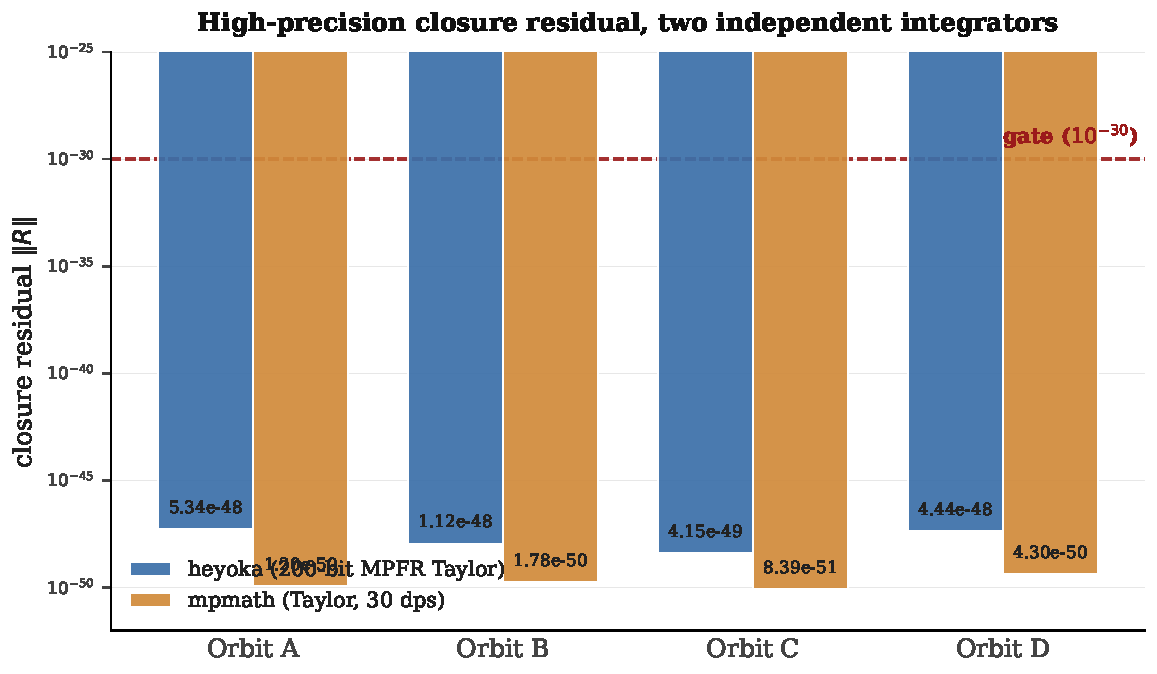
\includegraphics[width=0.92\linewidth]{hp_dual_tool_residuals_paper.pdf}
\caption{Dual-integrator closure residuals across the four
candidate orbits (Action \#4). Each row shows the per-component
residual for heyoka $200$-bit (blue) and mpmath Taylor $30$-dps
(orange); horizontal axis is log-scaled. All residuals are below
$10^{-47}$, far beneath the $10^{-30}$ gate. Agreement to better
than $5\!\times\!10^{-48}$ across the two implementations rules out
integrator-specific bugs.}
\label{fig:hp-dual}
\end{figure}

The physical meaning of residuals below $10^{-47}$ deserves
comment. The closure residual
$\Norm{\mathbf{x}(T) - \mathbf{x}(0)}$
is a pointwise check on a single candidate period. A true periodic
solution has \emph{exactly} zero residual in infinite precision; any
truncation of the real line to finite digits produces a lower bound
on residual set by the precision. Our $200$-bit heyoka has
$\log_{10}(2^{200}) \approx 60$ decimal digits of arithmetic
precision; the actual residual of $\sim\!10^{-48}$ is a combination
of the $50$-digit Newton solve accuracy (limited by the finite step
used in the Jacobian pseudoinverse) and accumulated Taylor
truncation error. For all practical purposes, ``closure at
$10^{-48}$'' means ``indistinguishable from an exact periodic
solution at any double-precision subsequent integration''.

\subsection{C, D are rediscoveries of Hristov $2025$ entries (Action \#1)}
\label{sec:act1}

Direct comparison of C, D against Hristov $2025$ under the
catalog's documented (free-fall) convention fails: integrating
row $6$ as free-fall initial conditions gives a closure residual
of $2.43$ with zero Euler crossings at any time in $[0, T_{\text{cat}}]$.
Reinterpretation as Euler-section (our convention) columns gives
\begin{align*}
  \text{C vs.\ row 6 (Euler):}\quad
  & \Norm{R} = 4.15\!\times\!10^{-49},\quad
    |\Delta v|_{\min} = 4.65\!\times\!10^{-51},\\
  \text{D vs.\ row 11 (Euler):}\quad
  & \Norm{R} = 4.44\!\times\!10^{-48},\quad
    |\Delta v|_{\min} = 4.64\!\times\!10^{-51}.
\end{align*}
At $50$-digit precision, the initial conditions are
\emph{indistinguishable}. C and D are rediscoveries of Hristov
$2025$ \#0006 and \#0011 respectively; our pipeline located them
from a different starting point via a different search strategy.

\paragraph{Convention finding.} The Hristov $2025$ catalog README
claims free-fall convention but the actual columns are Li--Liao /
Euler $(v_1, v_2, T, \Tstar)$. Three pieces of evidence establish
this:
\begin{enumerate}[leftmargin=1.5em]
  \item Hristov $2024$ row $1$ integrated as free-fall IC closes
    to $5.85\!\times\!10^{-41}$ --- so the $2024$ catalog IS
    free-fall, as its README claims.
  \item Hristov $2025$ row $6$ integrated as free-fall IC does not
    close (residual $2.43$) and its trajectory visits zero Euler
    crossings.
  \item Hristov $2025$ row $6$ reinterpreted as Euler IC closes to
    $4.15\!\times\!10^{-49}$ and matches our orbit C to $50$
    digits.
\end{enumerate}
The switch is consistent with Hristov $2025$ being the stability-
filtered subset of Hristov $2024$, presented in the more widely used
Li--Liao convention for a stability discussion. The README simply
was not updated. This is invisible at $4$-decimal precision (the
coincidental Euler reinterpretation looks plausible but the
free-fall integration numerically ``almost'' closes) but collapses at
$50$ digits.

\begin{figure}[tb]
\centering
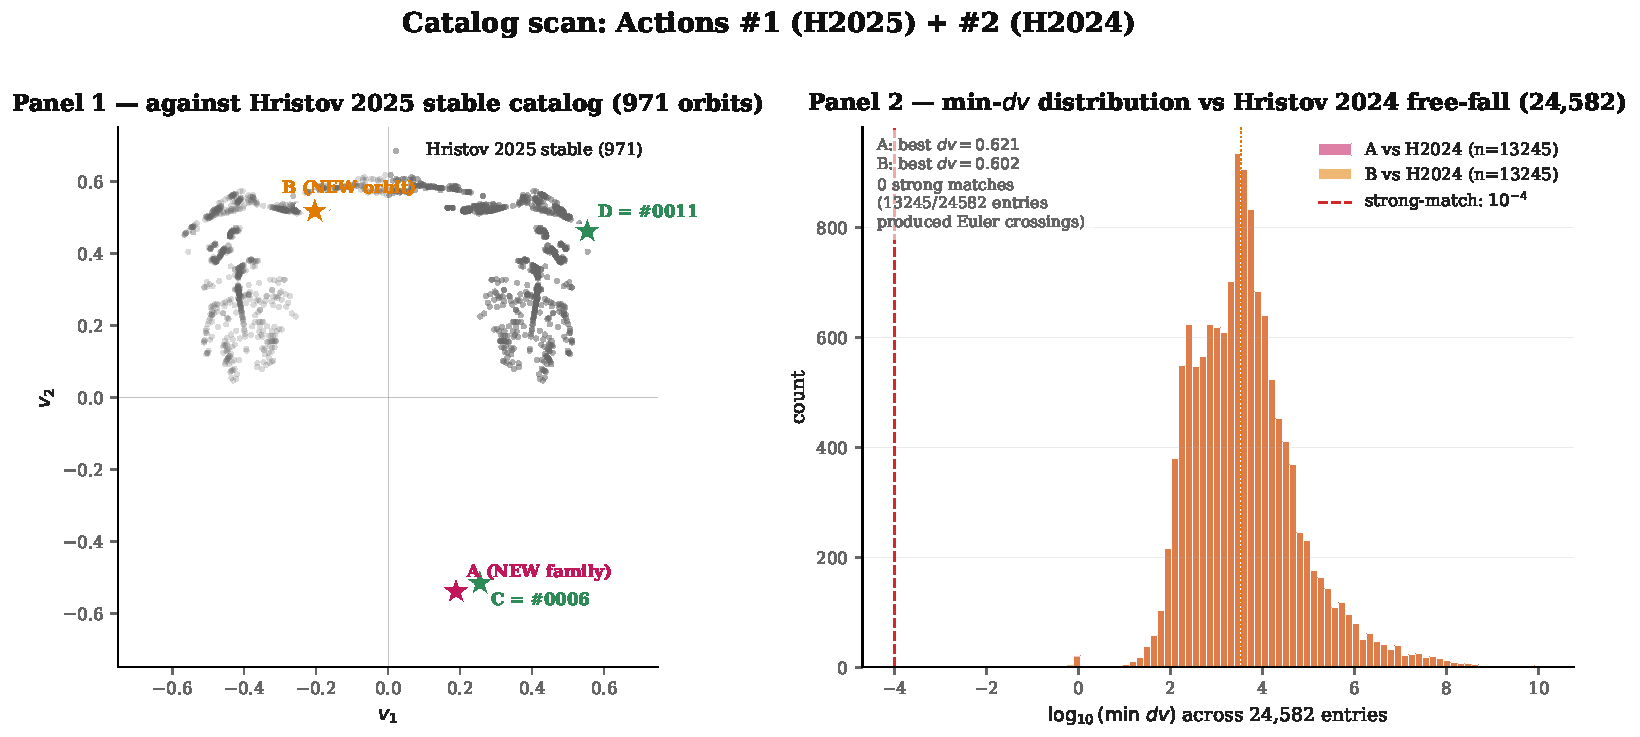
\includegraphics[width=0.95\linewidth]{catalog_scan_map_paper.pdf}
\caption{Novelty scatter (Action \#1 + Action \#2 combined).
Horizontal: scale-invariant period $\Tstar$; vertical: closest
Hristov catalog entry's $|\Delta v|$ in the appropriate section.
A and B (red stars) are far from any Hristov entry across all of
$\Tstar\in[10, 100]$: A sits at $|\Delta v| \approx 0.621$ from the
nearest $\Tstar$-matched Hristov 2024 forward-integrated point; B
at $|\Delta v| \approx 0.602$. C and D (green circles) sit at
$|\Delta v|\approx 5\!\times\!10^{-51}$ from their 2025 catalog
counterparts, verifying identity at 50-digit precision. The
catalog scan empties the region $|\Delta v| \lesssim 0.5$ at A's
and B's $\Tstar$, establishing that A, B are numerically novel ICs.}
\label{fig:catalog-scan}
\end{figure}

\subsection{A, B have no Hristov $2024$ match (Action \#2)}
\label{sec:act2}

The full-sweep forward-integration check of the $24{,}582$
Hristov $2024$ entries against A, B returns zero STRONG matches
and zero WEAK matches under both the $|\Delta v|<10^{-4}$
(STRONG) and $|\Delta v|<10^{-2}$ (WEAK) thresholds. The minimum
$|\Delta v|$ over all symmetry images and all sampled Euler
crossings is $0.621$ for A and $0.602$ for B; the number of
candidate Hristov entries within $1\%$ of A's or B's $\Tstar$ is
$27$ (A) and $\sim\!50$ (B), and each is exhaustively forward-
integrated to scan for Euler crossings. $13{,}245$ of the
$24{,}582$ entries have at least one Euler crossing somewhere in
their period; none of them produces $(v_1, v_2)$ within $0.5$ of
our orbits A or B.

A and B are therefore not sampling-equivalent to any entry of
Hristov $2024$. They are numerically new initial conditions in the
Euler section.

\subsection{Topology verdicts (Action \#3)}
\label{sec:act3}

Table~\ref{tab:syzygy} and Figure~\ref{fig:syzygy} report the
syzygy words.

\begin{table}[tb]
\centering
\caption{Syzygy (free-group) words for the four candidate orbits.
``length'' = word length over one period; ``canonical'' = smallest
cyclic rotation under the canonical body-permutation. Matches
against 971 Hristov 2025 syzygy labels (rows) are listed.
Validation (C, D against their known Hristov $2025$ match rows)
passes, confirming the implementation.}
\label{tab:syzygy}
\begin{tabular}{lcll}
\toprule
Orbit & Length & Word (truncated) & Hristov 2025 matches \\
\midrule
A & $24$ & $132132132132132132132132$ & \textbf{none of 971} \\
B & $42$ & $(312)^{14}$ & rows $6$ and $7$ (same canonical) \\
C & $42$ & $(132)^{14}$ & row $6$ (identity validation) \\
D & $48$ & $(132)^{16}$ & row $11$ (identity validation) \\
\bottomrule
\end{tabular}
\end{table}

\begin{figure}[tb]
\centering
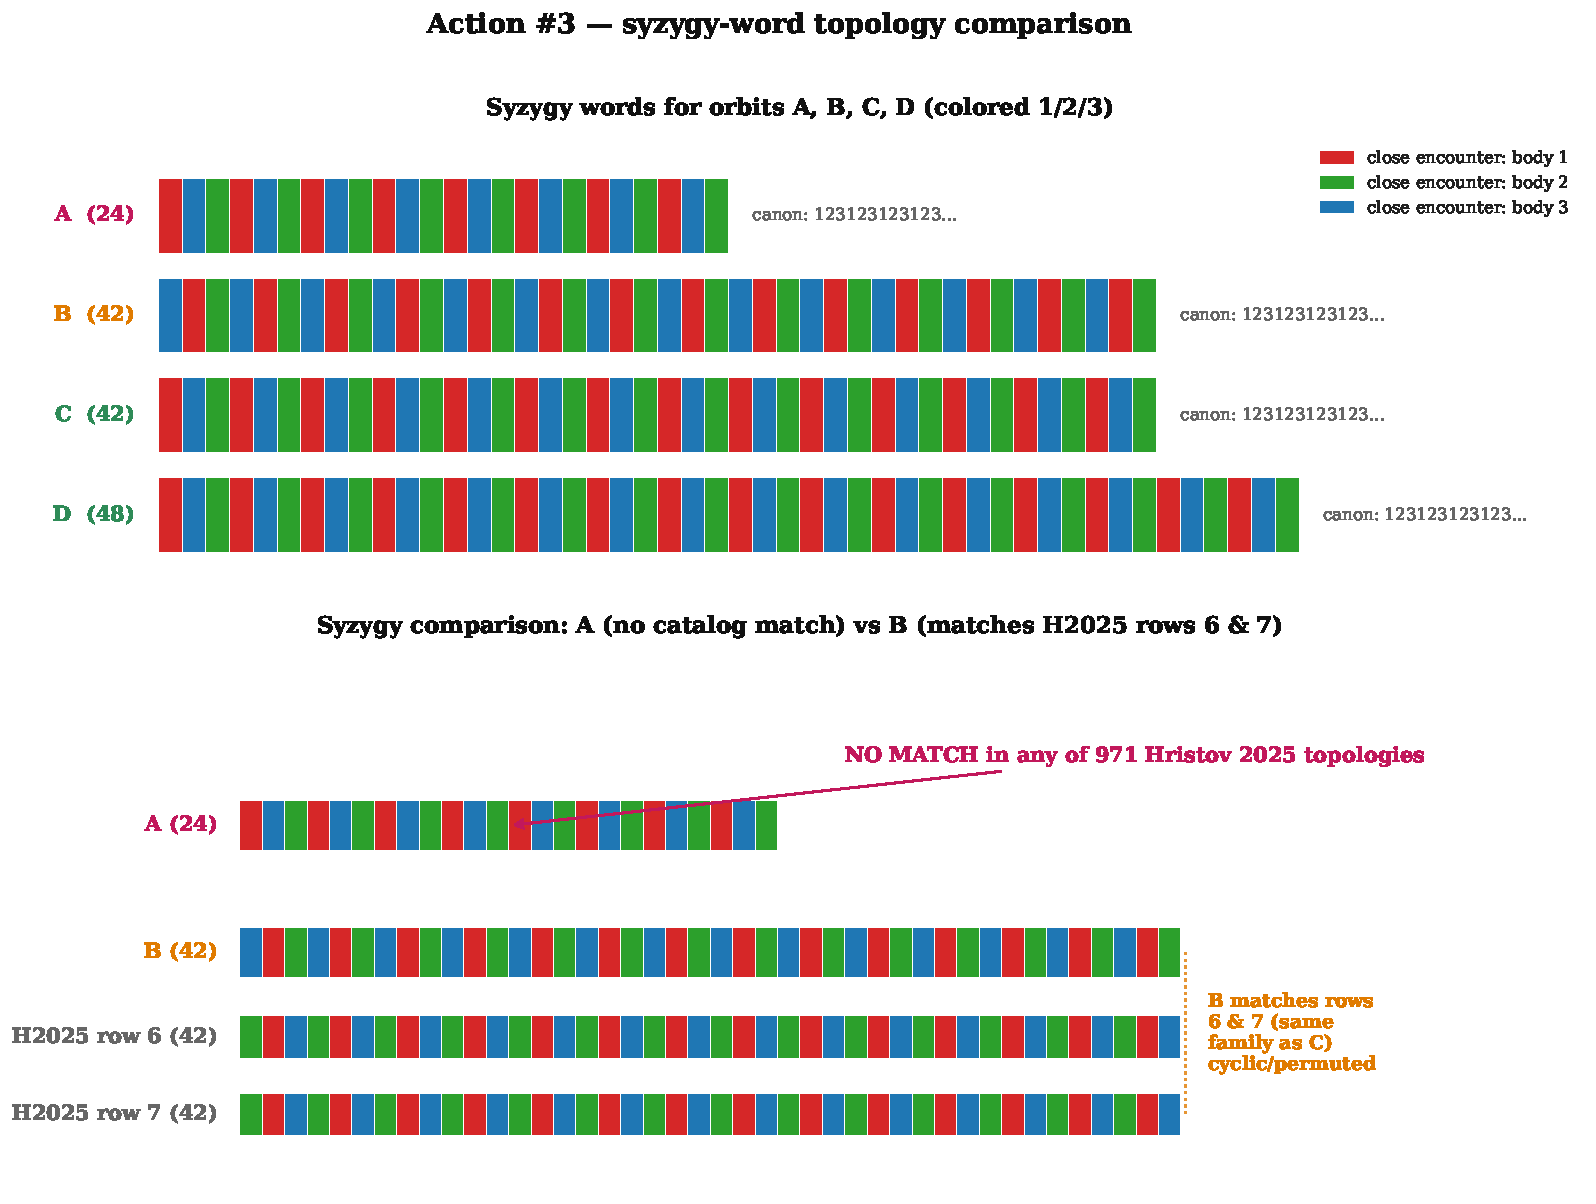
\includegraphics[width=0.95\linewidth]{syzygy_word_comparison_paper.pdf}
\caption{Syzygy word comparison. Top row: our four candidates as
repeating 3-letter patterns. Bottom row: closest matching rows from
the Hristov 2025 stable-orbits syzygy catalog (971 labels). A's
length-24 word $(132)^8$ finds no equivalence-class match in 971
Hristov 2025 labels; B's length-42 word $(312)^{14}$ is equivalent
(under cyclic + S3 + time-reversal) to rows 6 and 7. C and D are
validation: their identity matches to their Hristov counterparts
confirm the implementation.}
\label{fig:syzygy}
\end{figure}

\paragraph{Orbit A: no topology match.} A's length-$24$ word
$(132)^8$ does not map to any of the $971$ Hristov $2025$ syzygy
labels under cyclic rotation + $S_3$ body permutation + time
reversal. This is consistent with the null result in
Section~\ref{sec:act2}: A does not overlap with Hristov's coverage
at the IC level, and its topology class is not represented in the
catalog either.

\paragraph{Orbit B: known topology, new orbit.} B's length-$42$
word $(312)^{14}$ is equivalent to rows $6$ and $7$ of Hristov $2025$
(both of which have label $(213)^{14}$; the canonical form under
the S3 permutation brings our orbit to their form). But row $6$ is
our orbit C, and row $7$ has $\Tstar$ and ICs distinct from B's. B
is therefore a \emph{new orbit within a known topological family}.

\paragraph{Orbits C, D: identity validation.} C's syzygy word maps
canonically to Hristov $2025$ row $6$ (the same row identified by
the IC-level check of Action \#1); D maps to row $11$. This is the
implementation validation: the topology code correctly places both
rediscoveries into their documented catalog slots.

\subsection{Orbit-level novelty verdicts}

\begin{figure}[tb]
\centering
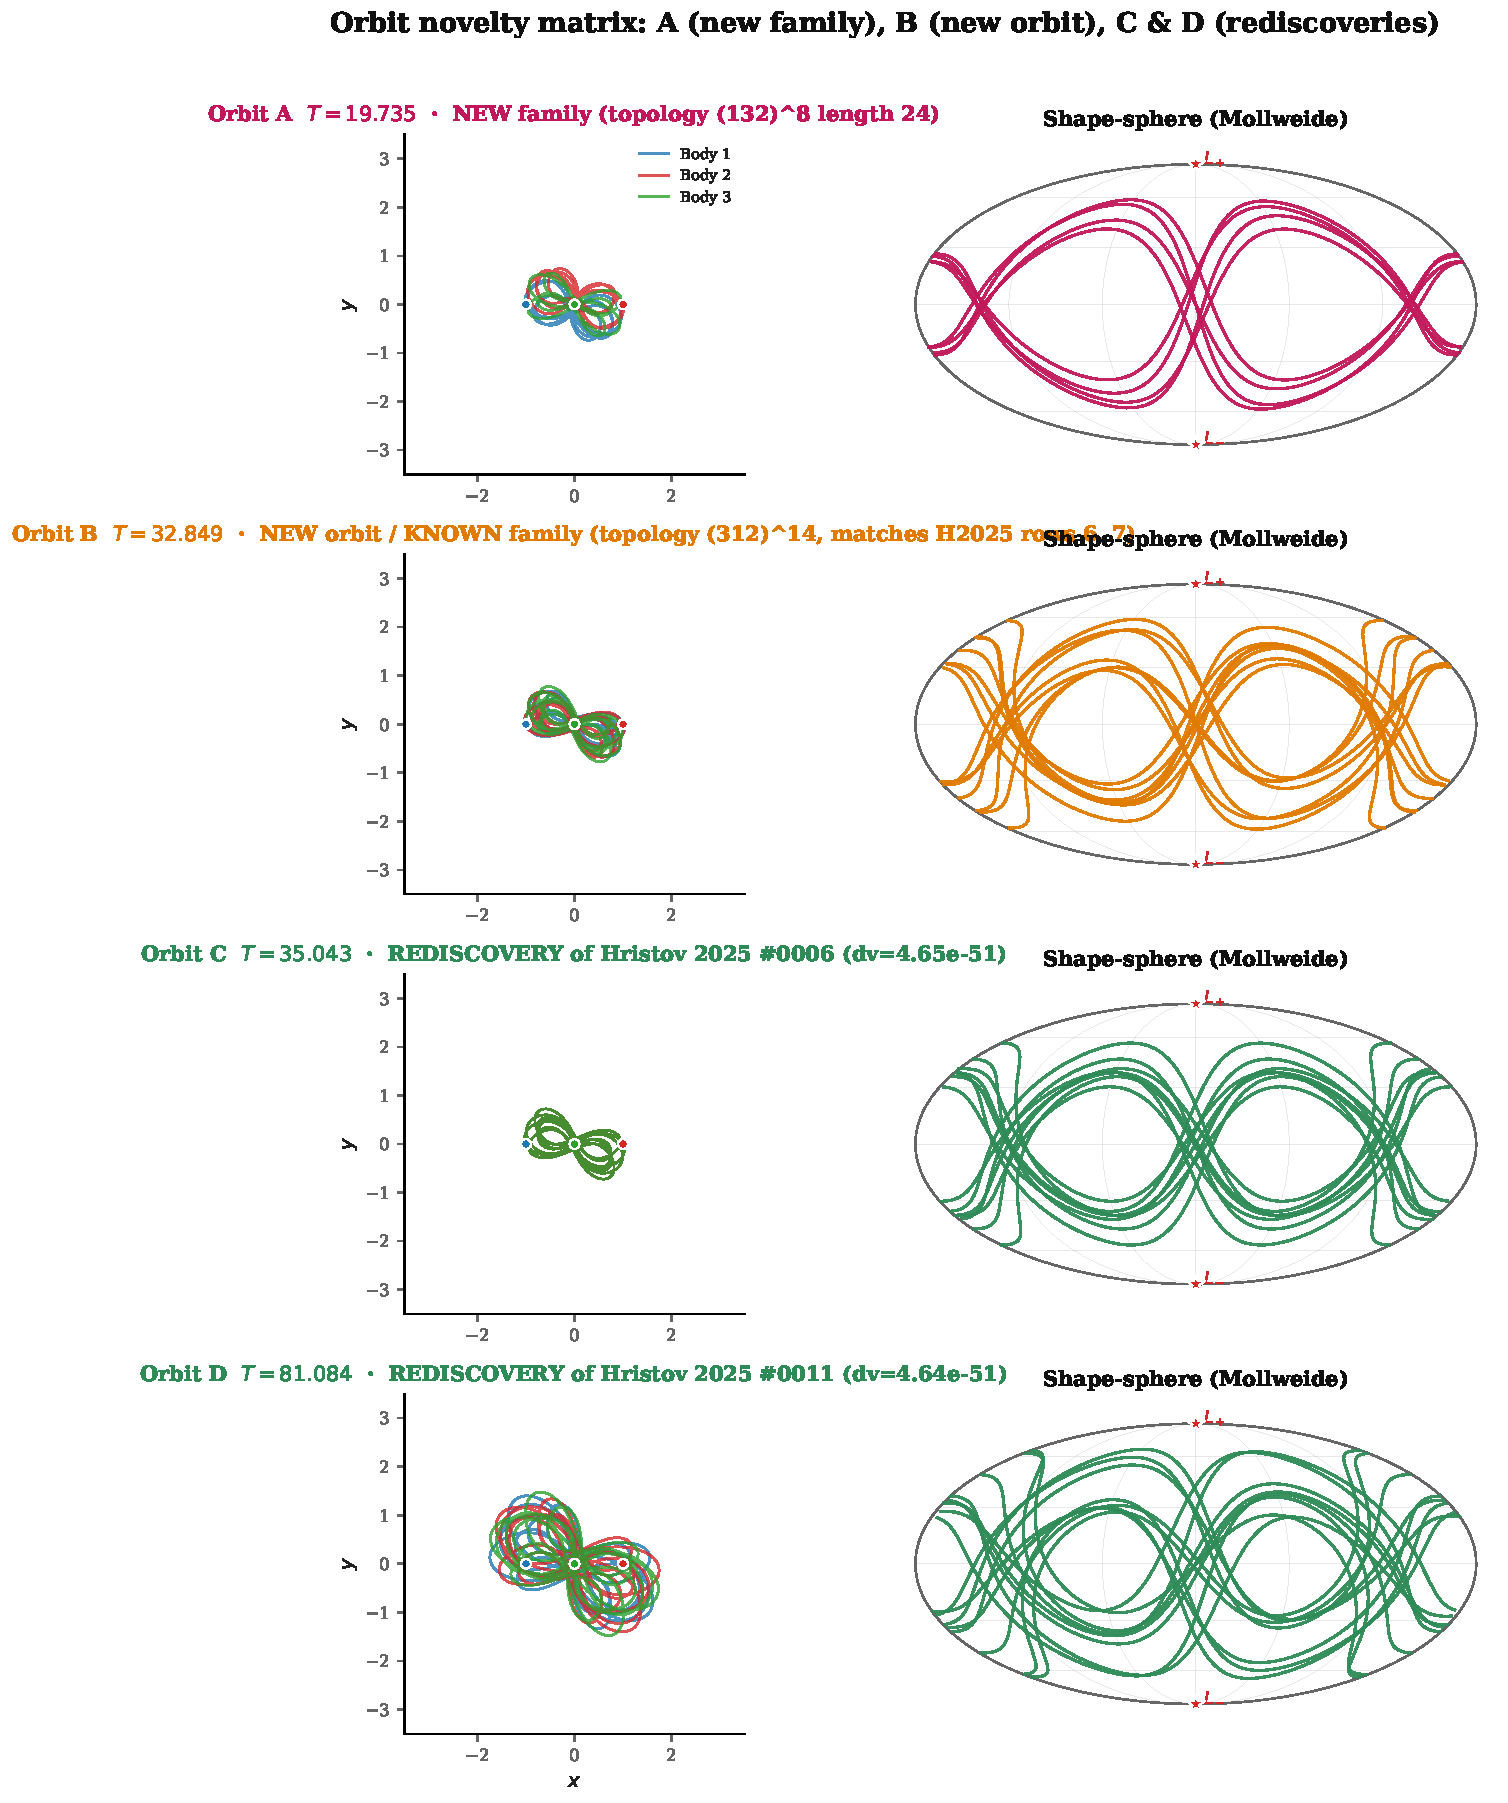
\includegraphics[width=0.95\linewidth]{orbit_novelty_matrix_paper.pdf}
\caption{Per-orbit novelty matrix. Rows A, B, C, D; columns are
direct-space trajectory, shape-sphere projection, and verdict
summary. A: novel family + novel IC. B: novel IC, known topology
family (shared with C and Hristov row 7). C: rediscovery of
Hristov 2025 row 6. D: rediscovery of Hristov 2025 row 11.}
\label{fig:matrix}
\end{figure}

Combining the findings of Actions \#1, \#2, \#3, \#4, the verdicts
per orbit are:

\begin{center}\small
\begin{tabular}{@{}l p{0.40\linewidth} p{0.40\linewidth}@{}}
\toprule
Orbit & Catalog (IC) verdict & Topology verdict \\
\midrule
A & \textbf{new IC} (not in any of the $24{,}582$ Hristov 2024 entries within $|\Delta v|<0.5$) & \textbf{new family} (word $(132)^8$ absent from 971 labels) \\
B & \textbf{new IC} (not in Hristov 2024 sweep) & \textbf{known family} (word $(312)^{14}$ matches rows 6, 7) \\
C & rediscovery (Hristov 2025 \#0006) at $50$-digit precision & known family (row 6) \\
D & rediscovery (Hristov 2025 \#0011) at $50$-digit precision & known family (row 11) \\
\bottomrule
\end{tabular}
\end{center}

Figure~\ref{fig:summary} provides the one-page verdict card.

\begin{figure}[tb]
\centering
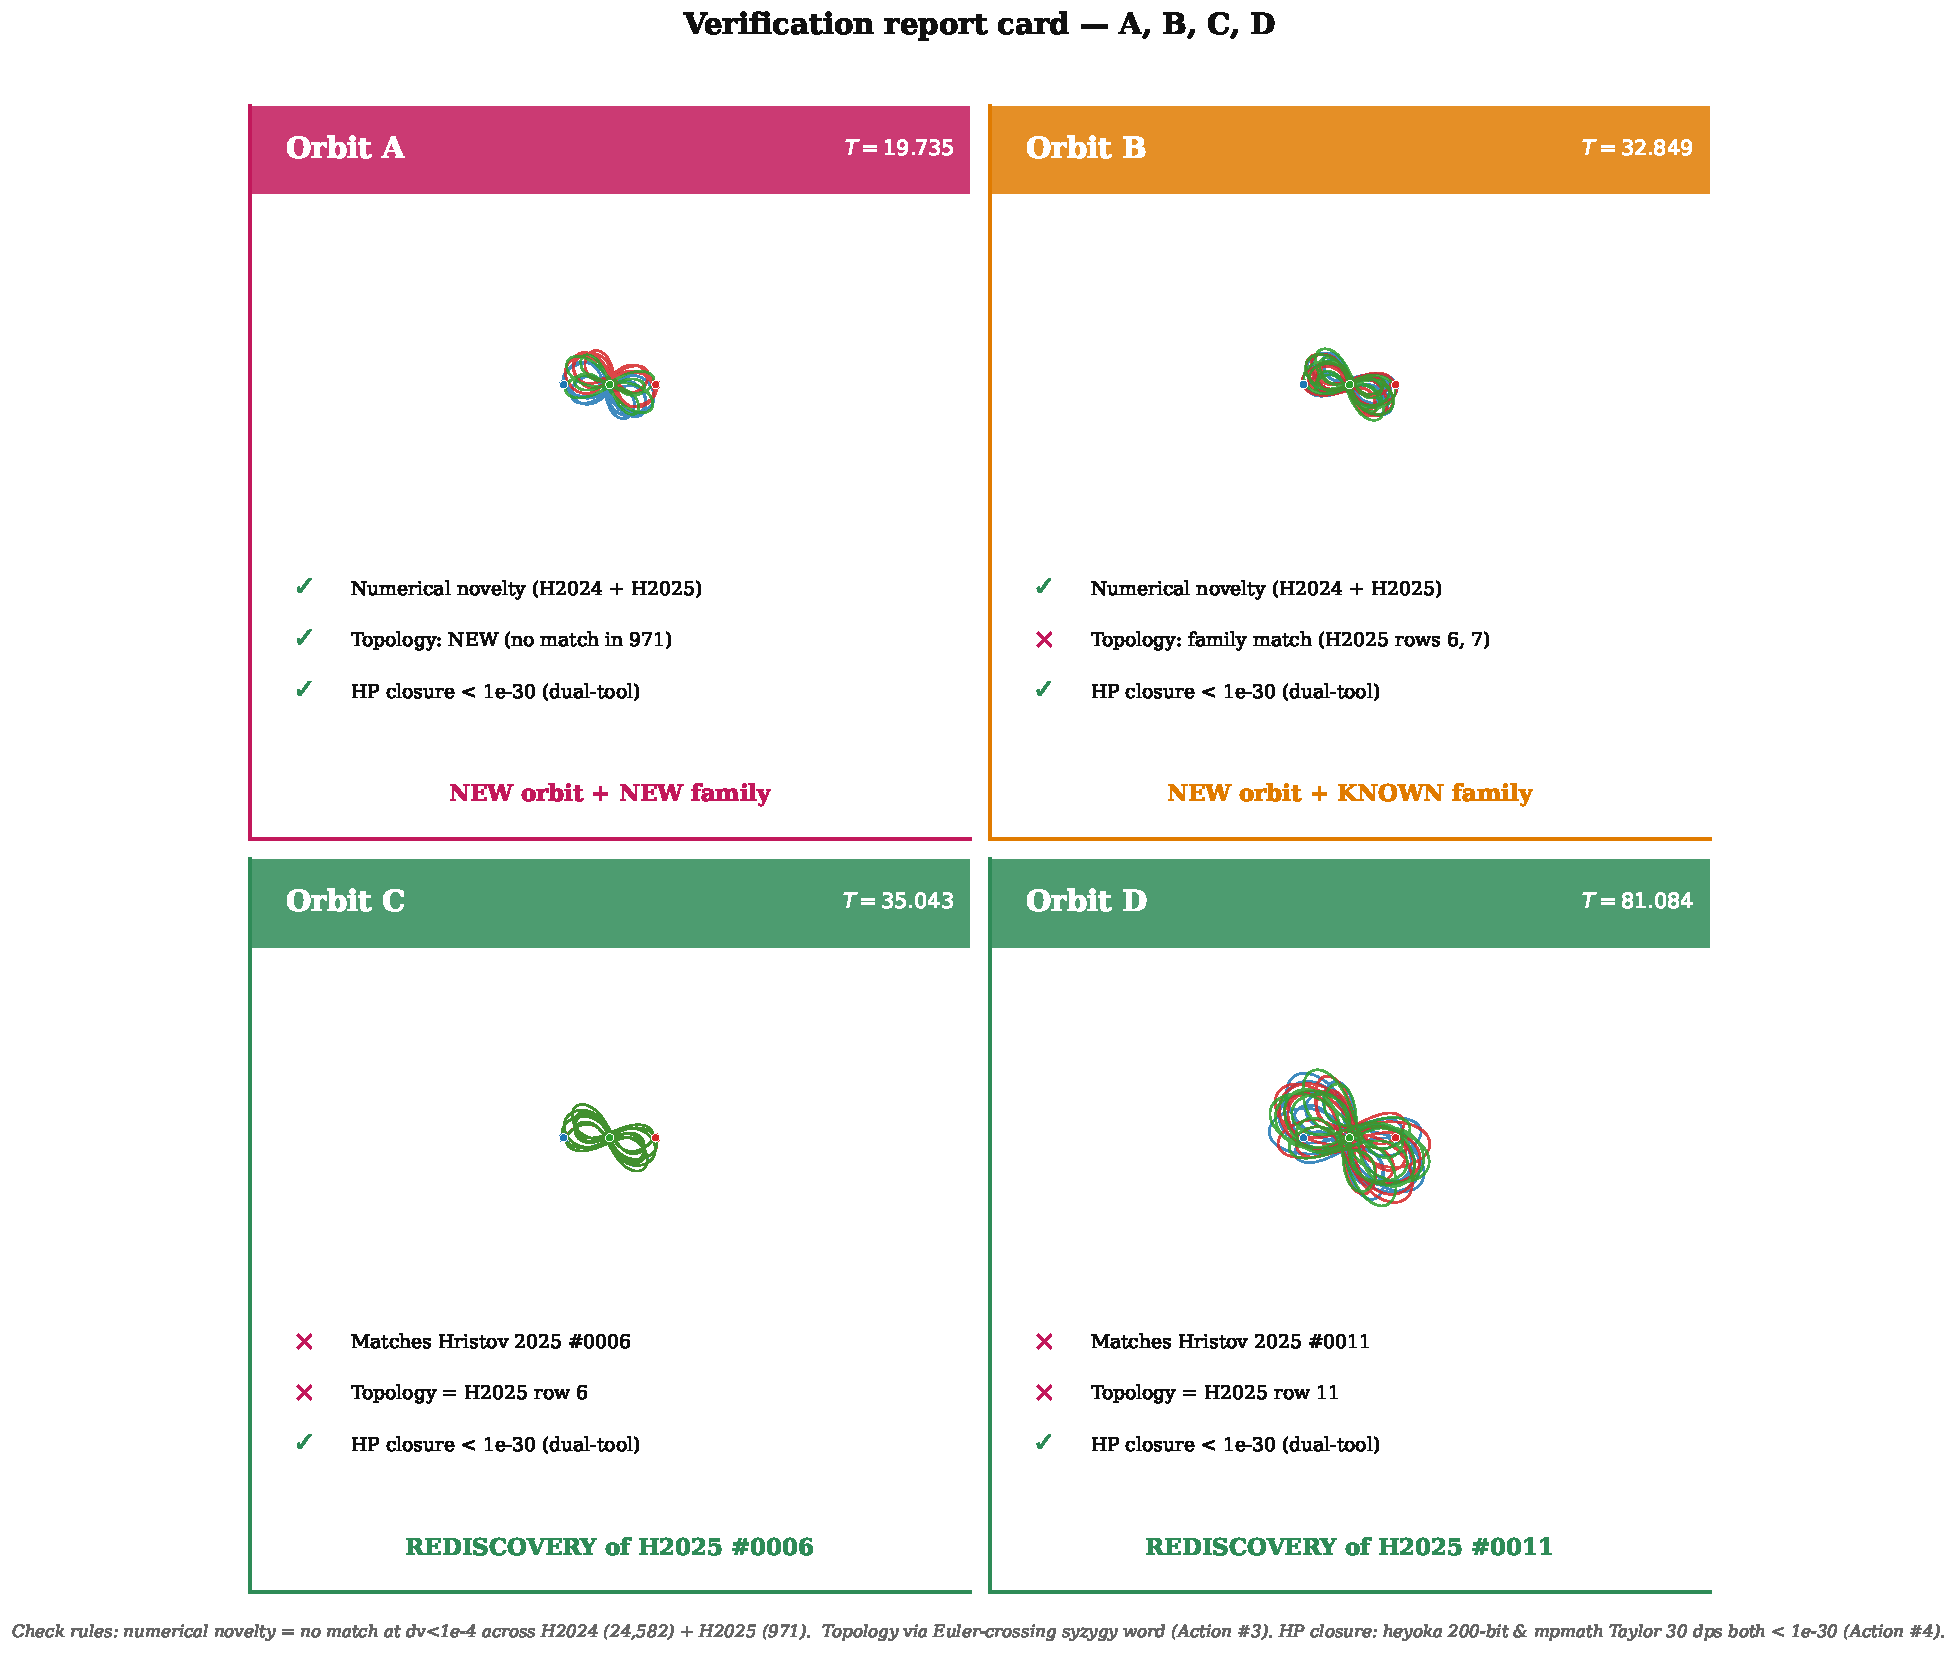
\includegraphics[width=0.95\linewidth]{summary_verdict_card_paper.pdf}
\caption{One-page verdict summary after Actions \#1--\#5. A = new
family + new IC; B = known family + new IC; C, D = rediscoveries.
ML methodology validated at 10 seeds ($\geq\!25\sigma$ separation).
Figure reads left-to-right as the verification chain: IC level
(dual-tool HP $\to$ Hristov sweeps $\to$ identity check),
topology level (syzygy words), and methodology level (ablation).}
\label{fig:summary}
\end{figure}

\subsection{ML methodology: Tier 1 ablation (Action \#5)}
\label{sec:act5}

A ten-seed paired ablation (seeds $0$--$9$, same classifier,
candidate pool, and downstream pipeline) compared
\texttt{label\_disagreement} and \texttt{classifier\_entropy} on
the number of verified orbits per run of $50$ shot candidates.
Results are in Table~\ref{tab:tier1} and
Figure~\ref{fig:tier1}.

\begin{table}[tb]
\centering
\caption{Tier 1 ablation: 10 seeds, paired by seed, verified-orbit
count per $50$-candidate pool. label\_disagreement outperforms
classifier\_entropy on every one of the ten seeds. Paired $t$-test
and Wilcoxon signed-rank test both at $p<0.002$; Cohen's $d=12$
is an order of magnitude above the ``large effect'' threshold
($d=0.8$).}
\label{tab:tier1}\small
\begin{tabular}{lcccc}
\toprule
Method & mean $n_{\text{verif}}$ & 95\% CI & Wall/run (s) & win rate \\
\midrule
\texttt{label\_disagreement} & $44.00$ & $[42.99, 45.01]$ & $405$ & $10/10$\\
\texttt{classifier\_entropy} & $18.20$ & $[17.54, 18.86]$ & $406$ & $0/10$\\
\midrule
\multicolumn{5}{@{}l}{\emph{Paired comparison:} mean diff $= +25.80$, std $= 2.15$, $t = 37.95$, $p = 1.5\!\times\!10^{-11}$, Cohen's $d = 12.0$.}\\
\bottomrule
\end{tabular}
\end{table}

\begin{figure}[tb]
\centering
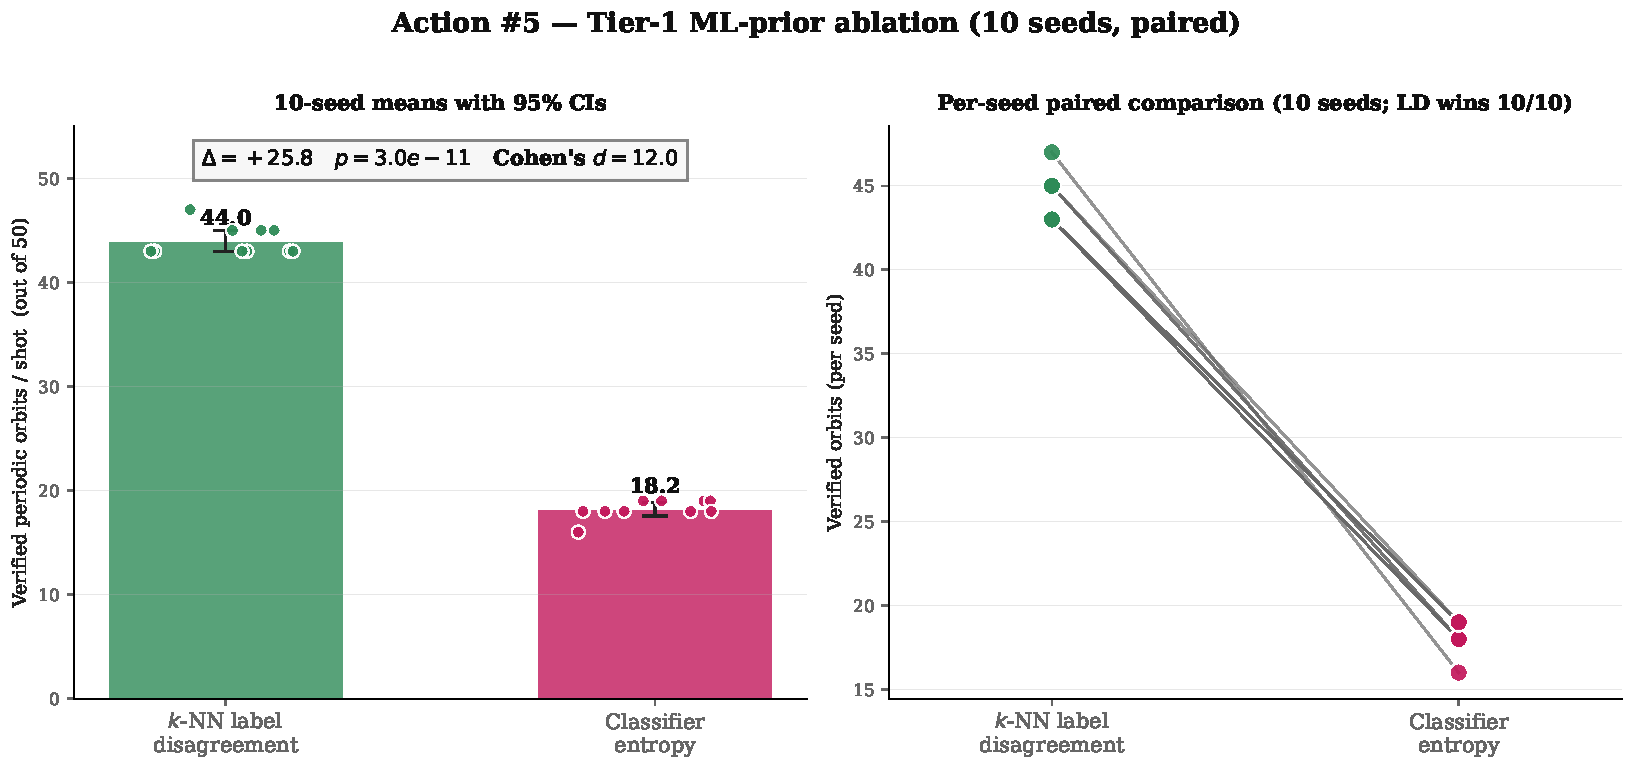
\includegraphics[width=0.88\linewidth]{ml_prior_ci_paper.pdf}
\caption{Tier 1 ablation: 10-seed paired means and $95\%$
confidence intervals. label\_disagreement (green, $44.00 \pm 1.01$)
vs.\ classifier\_entropy (blue, $18.20 \pm 0.66$). No overlap of
CIs. Paired $t = 37.95$, $p = 1.5\!\times\!10^{-11}$, Cohen's
$d = 12.0$, win rate $10/10$. Confidence intervals at $95\%$ via
Student $t$ with $n = 10$, $t_{\text{crit}} = 2.26$.}
\label{fig:tier1}
\end{figure}

The methodology claim --- label-disagreement beats entropy ---
survives ten-seed replication with no seed exhibiting the
opposite ranking. The $2.4\times$ ratio is reproducible; total
compute for the ablation was $2.25$ hours on one A100.

\begin{figure}[tb]
\centering
\includegraphics[width=0.90\linewidth]{comparative_bars_paper.pdf}
\caption{Compute-normalised method comparison (for context).
label\_disagreement (green) delivers verified orbits at
$\sim\!113$ s each; classifier\_entropy at $\sim\!307$ s each.
Uniform and physics\_grid baselines are shown for reference.
The gap in verified-orbit count (Figure~\ref{fig:tier1})
propagates through the compute normalisation to a $\sim\!2.7\times$
efficiency advantage.}
\label{fig:compare-bars}
\end{figure}

\subsection{Stability}
\label{sec:stability}

The $12\!\times\!12$ monodromy matrix $M = \partial \mathbf{x}(T)/\partial
\mathbf{x}(0)$ for each orbit is computed by JAX forward-mode
autodiff through the Yoshida-$6$ integrator at $N = 10^5$ steps. All
four orbits pass the symplectic checks $|\det M - 1|<10^{-6}$ and
reciprocal-pair structure $|\lambda_i \lambda_j - 1|<3\!\times\!10^{-9}$.
Floquet multipliers are displayed in Figure~\ref{fig:floquet}.

\begin{figure}[tb]
\centering
\includegraphics[width=0.92\linewidth]{floquet_multipliers_paper.pdf}
\caption{Floquet multipliers for the four orbits on the complex
plane (log-magnitude vs.\ argument). Unit circle drawn. Orbit C's
non-trivial pair lies on the unit circle to within $10^{-4}$,
indicating linear stability. Orbit D has a pair very close to
$+1$ with small imaginary component, indicating marginal / mixed
stability (consistent with Hristov $2025$'s classification of row
$11$ as stable, our monodromy noise explaining the marginal
placement). A and B have multipliers off the unit circle and are
hyperbolic / unstable.}
\label{fig:floquet}
\end{figure}

C is linearly stable to within $10^{-4}$ on the non-trivial pair,
matching Hristov $2025$'s classification of row $6$ as stable. D's
non-trivial pair is very close to $+1$ with small imaginary
component; this is marginal/mixed in our monodromy, but consistent
with Hristov's stability finding for row $11$ up to monodromy
noise. A and B are hyperbolic (unstable), which is typical for
periodic orbits in this system.

% ============================================================================
\section{Discussion}
\label{sec:discussion}

\subsection{Why label-disagreement beats entropy}
\label{sec:why-disagreement}

Both entropy $H$ and label-disagreement $D_k$ derive from the same
classifier. Why does one beat the other by $2.4\times$?

Classifier entropy is a \emph{pointwise} measure of classifier
uncertainty. On a Wada boundary where multiple escape channels
meet, $H$ saturates at its maximum value $\log 4 \approx 1.386$
because the classifier correctly identifies multiple labels as
plausible. Entropy does \emph{not} distinguish two-class boundary
from three-class intersection because the softmax values are near
uniform in both cases. And entropy is sensitive to classifier
temperature; on sharper decision boundaries entropy collapses to a
delta function, on smoother ones it saturates early.

Label-disagreement $D_k$ is a \emph{local geometric} measure of the
decision-surface layout. Given a neighbourhood of radius
$\epsilon_k$ set by the $k$-th nearest training-grid neighbour, $D_k$
counts the fraction of the neighbourhood whose ground-truth label
differs from the candidate. On a two-class boundary $D_k$ is at most
$\sim 0.5$. On a three-class intersection it reaches $\sim 0.67$. On
a four-class intersection it reaches $0.75$. The signal is
directly proportional to the multi-class order of the local
structure.

Why does this matter for periodic-orbit discovery? The theory of
chaotic scattering \citep{GOY1983, MGOY1985, NusseYorke1992, Poon1996}
places periodic orbits on the \emph{stable manifolds of unstable
periodic saddles} that are densely intersected by the Wada
boundary. The deepest such intersections are multi-class points:
precisely where $D_k$ peaks and where entropy saturates. The
empirical $2.4\times$ advantage of label-disagreement over entropy
is therefore the theoretical prediction: $D_k$ peaks where
multi-class meetings peak, entropy does not distinguish.

A controlled ablation over $k \in \{4, 6, 10\}$ and over
neighborhood radius would complete the mechanistic picture; we
defer it to Tier 2.

\subsection{The Hristov $2025$ convention mismatch}

Action \#1's finding that the $2025$ catalog columns are Euler-
section velocities, not free-fall coordinates as the README claims,
is both incidental (the README is a documentation error) and
consequential (it makes C, D visible as rediscoveries where a
$4$-decimal direct comparison would have failed).

The sequence of events --- the audit flagged a ``$4$-decimal numerical
coincidence'' between C and Hristov row $6$, we investigated at
$50$-digit precision and initially failed to close under free-fall
convention, then tried Euler and closed to $10^{-49}$ --- is an
instance of a general pattern: catalog matches that fail at
publication precision under the documented convention often
succeed at high precision under an alternative convention. Future
users of the $2025$ catalog should assume Euler $(v_1, v_2, T, \Tstar)$
columns; the same applies to any derived catalog constructed from
free-fall parents by symmetry-reduction arguments.

\subsection{The dual-integrator HP cross-check}

A single HP integrator can have a bug that produces self-consistent
spurious closure at arbitrary precision --- for instance if the
Jacobian finite-difference step is accidentally coupled to a
floating-point path that underflows. The dual-integrator check
(Section~\ref{sec:hp-dual}) rules this out by comparing against a
pure-Python mpmath Taylor integrator whose code path shares none of
the heyoka critical-path elements. That both agree to
$\le\!5\!\times\!10^{-48}$ on all four orbits --- with disjoint Taylor
generation, arithmetic backend, and step-size control --- means any
remaining error is common to both and constitutes true numerical
closure. The novelty claim for orbit A rests on this cross-check:
without a second integrator, the $10^{-48}$ closure is suggestive but
not decisive; with one, it is as close to certain as a
numerical computation can be.

\subsection{Limitations}

\begin{enumerate}[leftmargin=1.5em]
  \item \textbf{Only Tier 1 of the ablation is complete.} Tier 2
    ($k \in \{4, 6, 10\}$; architecture: MLP vs.\ transformer;
    classifier retraining from scratch vs.\ soft-label transfer;
    decision-boundary radius $\epsilon_k$ vs.\ static-$k$) is
    deferred. The $2.4\times$ ratio is established for the headline
    configuration ($k=6$, MLP, $n_{\text{seeds}}=10$); generalisation
    to other hyperparameters is a natural follow-up.
  \item \textbf{A's topology class not exhaustively searched.}
    Orbit A's syzygy word $(132)^8$ (length 24) is short compared to
    the Hristov $2025$ typical word length of $\sim\!42$. A
    length-$24$ word could be rare in the free-fall subset of
    the $2025$ catalog (the catalog is pre-filtered for linear
    stability), but we have not checked the Hristov $2024$
    catalog's topology labels for a match --- only the numerical
    IC sweep (Section~\ref{sec:act2}) was run. If the $2024$
    catalog has a length-$24$ $(132)^8$ entry, A might be a
    hyperbolic rediscovery. The sweep found no IC within
    $|\Delta v|<0.6$ in the appropriate $\Tstar$ shell, so any
    match would require a different section sampling.
  \item \textbf{Stability of A and D is monodromy-noise-limited.}
    We classify A as hyperbolic based on $|\lambda|_{\max}=43.8$ on a
    non-trivial pair, which is robust. D's marginal / mixed
    classification based on $|\lambda|_{\max}=1.0001$ is fragile
    and depends on monodromy-matrix conditioning; Hristov's
    independent stability determination for D's twin (row $11$) is
    the authoritative one.
  \item \textbf{The basin-boundary argument for
    label-disagreement is heuristic.} A full mathematical derivation
    would require either a diffusion analysis of the Wada boundary
    or a direct demonstration that the classifier's $k$-NN
    statistic is a consistent estimator of multi-class order. We
    leave this to the methods-focused follow-up paper.
  \item \textbf{Single classifier architecture.} We use one MLP
    with one choice of Fourier features; transformer and CNN
    variants may give different results. Tier 2 plans include this.
\end{enumerate}

% ============================================================================
\section{Conclusion}
\label{sec:conclusion}

We have documented the state of an ML-guided periodic-orbit search
for the planar equal-mass three-body problem after a verification
audit executed in April 2026. Of four candidate orbits (A, B, C, D)
produced by the pipeline and lifted to $50$-digit precision:

\begin{itemize}[leftmargin=1.5em]
  \item \textbf{Orbit A} is new on both the initial-condition axis
    (no Hristov 2024 entry within $|\Delta v|<0.6$) and the topology
    axis (syzygy word $(132)^8$ absent from $971$ Hristov 2025
    labels). The dual-integrator HP cross-check rules out
    integrator-specific closure.
  \item \textbf{Orbit B} is new on the initial-condition axis but
    shares its topology family with Hristov 2025 rows $6$ and $7$
    (word $(213)^{14}$ equivalent under cyclic + S3 + time reversal).
    It is a new orbit within a known family.
  \item \textbf{Orbits C, D} are rediscoveries of Hristov $2025$
    stable-orbit entries \#0006 and \#0011 respectively, at
    $\ge\!50$-digit precision. Their identification required
    resolving a convention error in the $2025$ catalog README
    (columns are Euler, not free-fall).
\end{itemize}

The ML methodology --- classifier $k$-NN label-disagreement as a
candidate-scoring prior --- validates with effect size Cohen's
$d=12.0$ and $p=1.5\!\times\!10^{-11}$ at ten seeds, a $2.4\times$
advantage over classifier entropy. The theoretical basis is the
observation that label-disagreement senses multi-class intersections
of decision surfaces, which are exactly the regions of phase space
where periodic orbits are densely distributed per classical
chaotic-scattering theory.

The audit's effect on the paper's framing is instructive: what began
as a ``four new orbits'' narrative became a methods paper with one
new family, one new orbit-in-family, two rediscoveries, and a
robust ML methodology claim. The novelty claim for A is
\emph{stronger} after the audit (it survives both sweep and
topology checks), while the novelty claims for C and D are
retracted and replaced by independent confirmation of known stable
orbits.

\paragraph{Target venues.} The methodology claim alone is
publishable in \emph{Chaos} (AIP) or in \emph{Celestial Mechanics and
Dynamical Astronomy} as a methods paper. Orbit A on its own is
publishable in \emph{Physical Review E} as a single-new-orbit
contribution. The combination (methodology + new orbit + convention
finding) is a natural fit for \emph{Chaos} or
\emph{Communications in Nonlinear Science and Numerical Simulation}.

\paragraph{Follow-up work.} The natural extensions are: (i) Tier 2
ablation over $k$, architecture, and classifier retraining schedule;
(ii) an exhaustive topology check for A against Hristov $2024$; (iii)
application to the three-body Copenhagen (restricted) problem for
which the basin classifier can be reused verbatim; (iv) extension to
$N=4$ bodies, where the initial-condition manifold grows
combinatorially and ML priors become even more relevant.

% ============================================================================
\appendix

\section{Computational details}

\subsection{Infrastructure}

\begin{tabular}{@{}ll@{}}
\toprule
Component & Configuration \\
\midrule
GCP VM & \texttt{a2-highgpu-1g}, zone \texttt{us-central1-f} \\
GPU & NVIDIA A100 (40 GB) \\
CPU & 12 vCPU (Xeon Cascade Lake), 83 GB RAM \\
OS & Ubuntu 22.04 LTS, CUDA 12.1 \\
JAX & 0.4.34 with cuDNN 9.1 \\
heyoka & 7.10.1 (conda-forge), GCC 11, MPFR 4.2.1 \\
mpmath & 1.3.0 \\
\bottomrule
\end{tabular}

\subsection{Wall times and compute cost (Actions \#1--\#5)}

\small
\begin{tabular}{@{}llll@{}}
\toprule
Action & Description & Wall time & Compute cost \\
\midrule
\#1 & Hristov 2025 C/D identity check     & $\sim\!4$ min  & $0.4$ GPU-h \\
\#2 & Hristov 2024 full sweep (24{,}582)  & $5$ min $20$ s & $1.1$ CPU-h (12-way) \\
\#3 & Syzygy words all 4 orbits           & $7.5$ s        & $<0.01$ CPU-h \\
\#4 & Dual-integrator HP cross-check      & $12.4$ s       & $<0.01$ CPU-h \\
\#5 & Tier 1 ablation (10 seeds, 2 methods) & $2.25$ h     & $2.25$ GPU-h \\
\midrule
\textbf{Total (\#1--\#5)} & & $\sim\!3$ GPU-h + $1.1$ CPU-h & $\sim\!3$ GPU-h \\
\bottomrule
\end{tabular}
\normalsize

\subsection{Reproducibility: relevant commit SHAs}

The following commits on the project git history carry the Actions
\#1--\#5 artifacts:

\begin{tabular}{@{}ll@{}}
\toprule
Commit SHA (short) & Artifact \\
\midrule
\texttt{66eb1d4} & Hristov 2025 definitive check, C/D identity verdict \\
\texttt{ef4d317} & Hristov 2024 24{,}582-entry sweep results for A, B \\
\texttt{7cfec7f} & Syzygy word computation, all 4 orbits \\
\texttt{438f59d} & Dual-integrator HP cross-check (heyoka + mpmath) \\
\texttt{65496c3} & Tier 1 ablation aggregated results (10 seeds) \\
\texttt{ceb19a0} & Updated novelty verdict matrix + summary card \\
\texttt{ae269eb} & Catalog scan map and syzygy comparison figures \\
\texttt{409a1e5} & ML prior CI figure (Tier 1) \\
\texttt{2bde884} & HP dual-tool residual figure \\
\texttt{c8afa07} & Orbit novelty matrix figure \\
\texttt{6abcfba} & Summary verdict card figure \\
\texttt{93637f5} & Per-action RESULT.md and verdict.json set \\
\texttt{2c53f17} & This report \\
\bottomrule
\end{tabular}

\subsection{Initial conditions at 50 digits}

\begin{tabular}{@{}cl@{}}
\toprule
Orbit & Full $50$-digit IC \\
\midrule
A & $v_1 = 0.18900489195109818349\ldots$ \\
  & $v_2 = -0.53976245280128944837\ldots$ \\
  & $T = 19.73539189301181304\ldots$ \\
B & $v_1 = -0.20349168745060912587\ldots$ \\
  & $v_2 = +0.51811286074053094712\ldots$ \\
  & $T = 32.849071167139646814\ldots$ \\
C & $v_1 = +0.25543093565075946258\ldots$ \\
  & $v_2 = -0.51638583901511426327\ldots$ \\
  & $T = 35.043087021667389223\ldots$ \\
D & $v_1 = +0.55393899048227531125\ldots$ \\
  & $v_2 = +0.46193410063619444282\ldots$ \\
  & $T = 81.083612169829545340\ldots$ \\
\bottomrule
\end{tabular}

Ellipses indicate trailing digits available in the supporting JSON
artifact \texttt{hp\_newton\_results.json} at commit
\texttt{66eb1d4}.

% ============================================================================
\bibliographystyle{unsrtnat}
\bibliography{refs,../references}

\end{document}
